\begin{paragraph}{Primo Metodo}
Si vuole fittare i dati con seni e coseni di opportuna frequenza $k$
e fase da determinare (parametro di fit). Si definiscono allora:\\
  In ZonaI = $\{x<-b\}$, sia
        $$f^{even}_k(y) = \int_{-\infty}^{-b} | A\cos(kx+y)-\psi_k^{even}(x)| \mathrm d x $$
        $$f^{odd}_k(y) = \int_{-\infty}^{-b} | A\sin(kx+y)-\psi_k^{odd}(x)| \mathrm d x $$
  In ZonaIII = $\{x<-b\}$, sia
        $$g^{even}_k(y) = \int_{b}^{+\infty} |A\cos(kx+y)-\psi_k^{even}(x)| \mathrm d x $$
        $$g^{odd}_k(y) = \int_{b}^{+\infty} |A\sin(kx+y)-\psi_k^{odd}(x)| \mathrm d x $$
Si ha immediatamente che:
    $$ \theta^-_k = y \mbox{ t.c. } f_k(\theta^-_k) = 0 $$
    $$ \theta^+_k = y \mbox{ t.c. } g_k(\theta^+_k) = 0 $$
\end{paragraph}
Si troverà che:
    $$ \theta^+_k = -\theta^-_k = \theta_k $$
Quindi:
$$ \psi_k^{odd} = \begin{cases}
    A\sin(kx - \theta_k) & \mbox{in ZonaI} \\
    A\sin(kx + \theta_k) & \mbox{in ZonaIII} \\
\end{cases}
\quad
\psi_k^{even} = \begin{cases}
    A\cos(kx - \theta_k) & \mbox{in ZonaI} \\
    A\cos(kx + \theta_k) & \mbox{in ZonaIII} \\
\end{cases}
$$

\begin{paragraph}{Secondo Metodo}
Si considerino i punti $x = \pm 2\pi$, siano $y(\pm 2\pi)$ i valori degli autovettori
numerici in quei punti, separatamente pari e dispari. Si ha allora che:
$$ \begin{cases}
    y^{odd}(2\pi)   = \sin(k2\pi  + \theta_o^+)  & \Rightarrow \theta_o^+ = \arcsin(y^{odd}(2\pi)) - k2\pi\\
    y^{odd}(-2\pi)  = \sin(-k2\pi + \theta_o^-)  & \Rightarrow \theta_o^- = \arcsin(y^{odd}(-2\pi)) + k2\pi\\
    y^{even}(2\pi)  = \cos(k2\pi  + \theta_e^+)  & \Rightarrow \theta_e^+ = \arccos(y^{even}(2\pi)) - k2\pi\\
    y^{even}(-2\pi) = \cos(-k2\pi + \theta_e^-)  & \Rightarrow \theta_e^- = \arccos(y^{even}(-2\pi)) + k2\pi\\
\end{cases}$$
\end{paragraph}
Di seguito il plot del risultato\\
%% Sarebbe bello che stesse sulla stessa pagina
\begin{figure}[h]
  \centering
  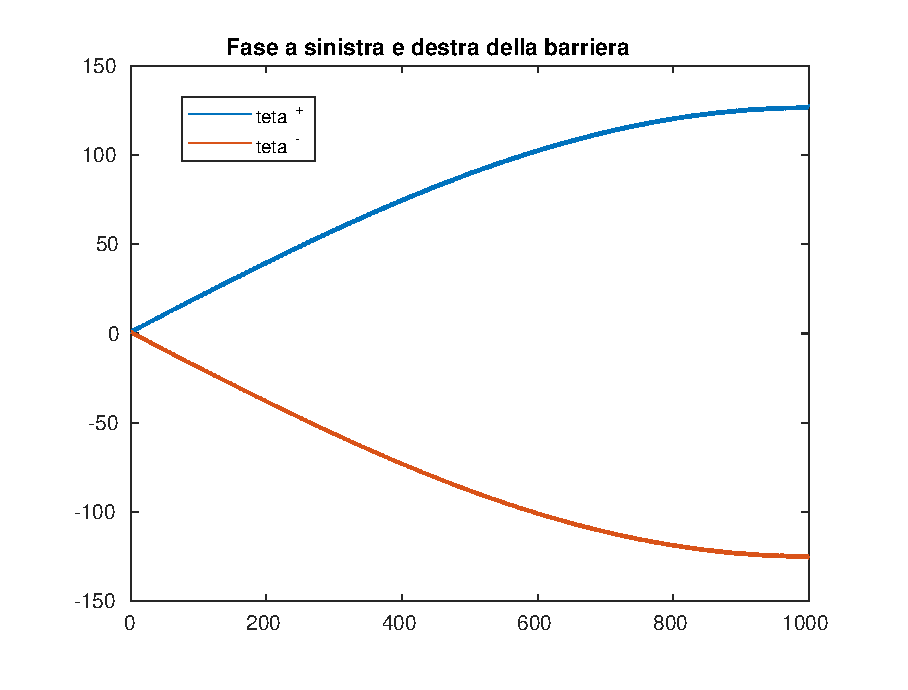
\includegraphics{fasi.eps}
\end{figure}
